\chapter{Data Sources and Methods}
\pdfcomment{provide information about ocean color data}
\pdfcomment{Explain how my processing chain differs from the NASA one}
\pdfcomment{make sure to explain how I add the ATL03 parameters to find the geoidal height}
\pdfcomment{mention the UTM grid reprojection steps if they're not mentioned.}
\section{Data Sources}
The following data sources were used as input to the 
\subsection{NASA ATL03}

The main source of data is NASA's ATL03 V005 data product \parencite{icesat2data}. ATL03 is a level 1 data product that consists of the precise latitude, longitude, and elevation for each received photon. As a level 1 data product, it has already undergone some processing by the Atlas Science Algorithm Software (ASAS) to correct for instrument errors, to classify photons as likely signal or noise for different surface types, and to correct for some geophysical effects including earth tides to provide provide measurements relative to the WGS-84 ellipsoid. 

Additionally, the data includes variables that allow for further corrections and adjustments to the tide-free geoid reference system. These additional variables include correction factors for the tide, ocean surface depression due to atmospheric pressure, and factors to convert the ellipsoidal elevation to a height relative to the tide-free geoid.

\subsection{GEBCO Global Grid}

The General Bathymetric Chart of the Ocean (GEBCO) is a global grid of topography and bathymetry at a 30 arc-second mesh resolution \parencite{gebco2021griddata}. GEBCO is assembled by compiling many different data sources, including mutli-beam sonar data, nautical charts, and satellite gravimetric measurements for deep-ocean bathymetry \parencite{gebcocookbook}. The elevation data is referenced to a vaguely-defined 'mean sea level'. The various data sets included in gebco are all assumed to be referenced to MSL, but some datasets referenced to chart datum are included. 

GEBCO has a limited accuracy and resolution, but it is the only available data source in many places in the world, so it is sometimes used as the best-estimate in very data-poor sites. However, the accuracy of GEBCO varies depending on the input data sources. In this project, the GEBCO elevation is used both to filter locations that \emph{may} contain valid bathymetry, and used as a prior guess to the bayesian updating approach. 

\subsection{GlobColour Daily secchi depth data}

The data from \parencite{Garnesson2019} is also linked to each transect to investigate the relationship between the

\section{Methodology}

To reach the end goal of incorporating ICESat-2 into GEBCO grids, first the lidar photon data for the area of interest is downloaded, processed into geoidal heights, subset to only include subsurface photons, find bathymetric signal within the subsurface data, interpolate into a 2D grid, then finally combine the interpolated ICESat-2 data with the resampled GEBCO grid within the area of interest. Then, for the test sites, the change in in the various error metrics between the naive bilinear interpolation is calculated. 

\subsection{Processing ATL03}
To download data for a specific site geographic area of interest is created, and this area is passed to the NSIDC download API to use for spatial subsetting. This allows spatial subsetting of the data download which reduces file size. The NSIDC API also allows subsetting by the variable name, so only the ATL03 variables that are relevant for this research are downloaded, which further reduces the file size for practical download and storage of the ATL03 data. 

The three variables that define the 3D location in the WGS-84 reference frame of each photon are \emph{h\_ph},\emph{lat\_ph}, and \emph{lon\_ph} are located in the \emph{heights} group within the ATL03 data structure. To use these variables for the purpose of bathymetric measurement, several other variables are required for processing. To transform the ellipsoidal elevation to the geoidal elevation, the two additive factors \emph{geoid} and \emph{geoid\_free2mean} are included in the download.

These correction factors are not provided for every single photon but are provided for each 20m segment because they vary at scales that are longer than the photon rate. To find the correct factor for each photon, we need to link the segment-rate variables to the photon rate variables. This is done using the python package Pandas \parencite{jeff_reback_2022_6408044,mckinney-proc-scipy-2010} which has many functions for manipulating time-series data. 

\subsection{Filtering ATL03 to subsurface returns}

The bathymetric signal that we are seeking to find is located in the shallow-water nearshore zone. Therefore, photons outside that zone need to be removed reduce processing time and eliminate false positives as much as possible. To reduce the downloaded transect data within the area of interest, the following filtering steps are applied to each transect \pdfcomment{Add figures For each of these steps}:

\begin{enumerate}
    \item For every photon, find the GEBCO depth at that location. Any photons with a GEBCO elevation between -50 and 3m are selected, and those outside of this region are culled from the data set. Points that are outside this range are assumed to be deeper than the maximum known depth detectable by ICESat-2 (38m per \citeauthor{Parrish2019}), or assumed to be on land. This provides a horizontal filtering along the transect. An example of this process can be seen in figure \ref{fig:gebco_filtering}
    
    \begin{figure}[h!]
        \centering
        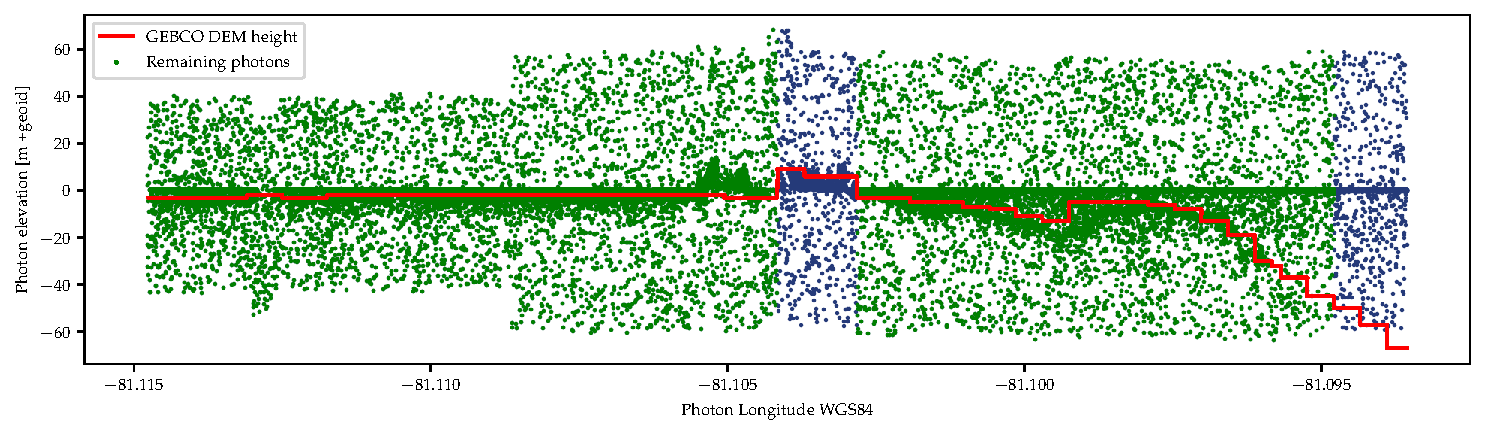
\includegraphics[width=\textwidth]{figures/methodology_gebco_filtering.jpg}
        \caption{The GEBCO data for the example transect, and the photons that are removed due to the GEBCO depth}
        \label{fig:gebco_filtering}
    \end{figure}

    \item To remove any high noise, cloud returns, or any remaining high land points not removed in step 1, any points more than 5m above the geoid are removed, based on the approach in \citeauthor{Ranndal2021}.
    \item The local sea-surface elevation $h_{sea}$ is calculated by taking the median elevation of photons that are classified as high-confidence sea surface photons. The water depth for each photon is then calculated. The standard deviation of the elevation high-confidence photons $\sigma_{h_{sea}}$ is also calculated to estimate the magnitude of the wave height at the time of the observation.
    \item Any points with a water depth greater than 40 meters, and points with an geoidal height  less than -40m are removed, based on the same assumption that they are too deep to by bathymetric points. 
    \item Any points that are higher than the ocean surface elevation + $max(\sigma_{hconf_oc},1)$ are removed. 
    
    
    The results of steps 3-5 \pdfcomment{check} are shown in figure \ref{fig:vert_filtering}
    \pdfcomment{fix legend on this graph}
    \begin{figure}[h!]
        \centering
        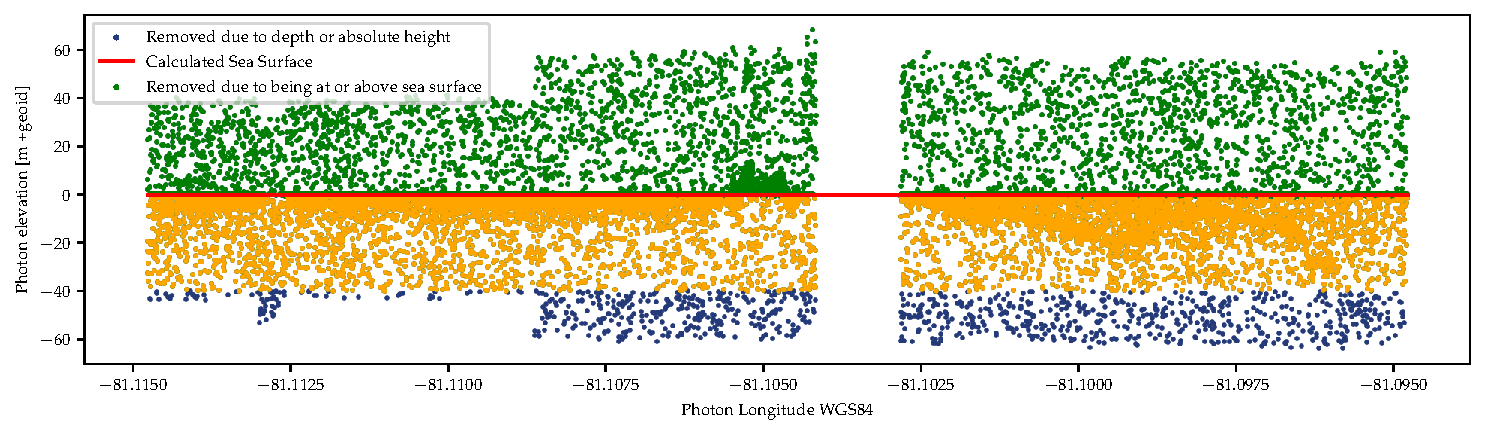
\includegraphics[width=\textwidth]{figures/methodology_sealvl_filtering.jpg}
        \caption{Vertical point filtering based on the local sea surface elevation}
        \label{fig:vert_filtering}
    \end{figure}
\end{enumerate}

After these filtering steps, the resulting subsurface photons for this example transect are shown in figure \ref{fig:remaing_photons}

\begin{figure}[h!]
    \centering
    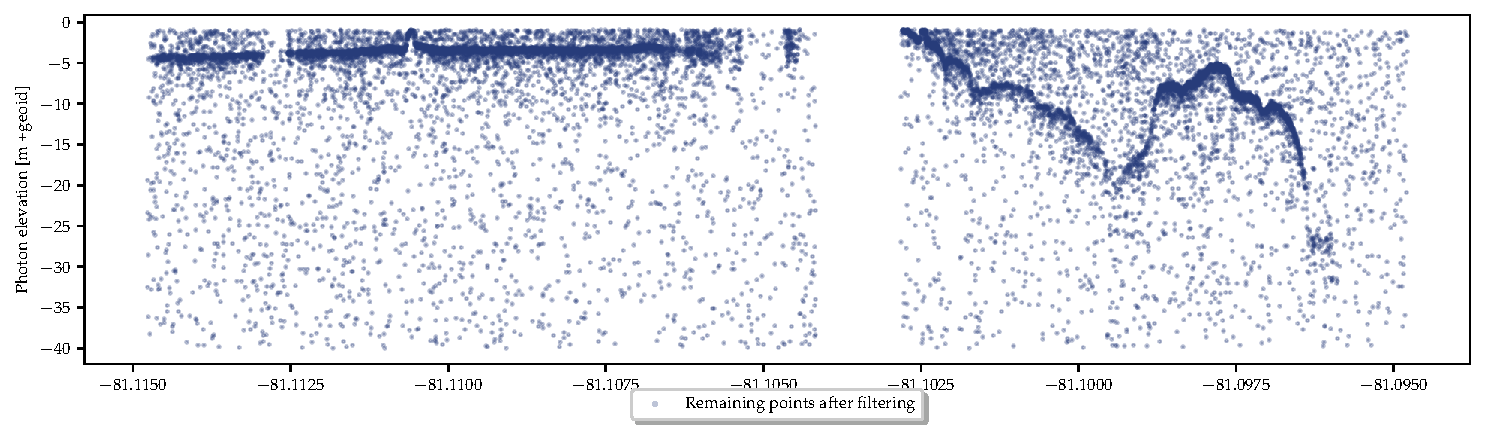
\includegraphics[width=\textwidth]{figures/methodology_reminaing_after_filtering.jpg}
    \caption{Subsurface photons found resulting after the filtering process}
    \label{fig:remaing_photons}
\end{figure}

\subsection{Bathymetric Signal Finding}

The filtering steps reduce the dataset to just photon that are in the subsurface zone. To determine if there is bathymetric signal present, further processing is required. Some proposed methods for separating bathymetric signal photons from noise are explained in section \ref{subsec:denoising}. For this project\pdfcomment{reword?}, a new method is proposed based on a Gaussian Kernel Density Estimation (KDE) function. A function is created that returns the maximum kernel density, and the Z location at which it occurs. $$ f(\hat{z}_{window}) \rightarrow kde_{max},z_{kde_{max}} $$ Figure \ref{fig:kdefunc} shows the KDE function as applied to an example window, and the resulting kernel density plot. The KDE function is highly influenced by the \emph{Bandwidth} parameter. For this implementation, the Scott method \parencite{Scott2015} is used to estimate the required bandwidth based on the distribution of the data. 

This function is applied on a rolling basis to a window of 200 points. This function returns a value for every single point along the transect, including in areas that do not have any noticeable signal. The kernel density value gives an indication of the strength of the peak. To reject the locations where the signal is weak, any points with a KDE value of less than the median value $$ kde_{50} $$ \pdfcomment{maybe just less than median? that decreases RMS error at the florida site} are assigned an NaN value and are dropped from the analysis.

\begin{figure}[htbp]
    \centering
    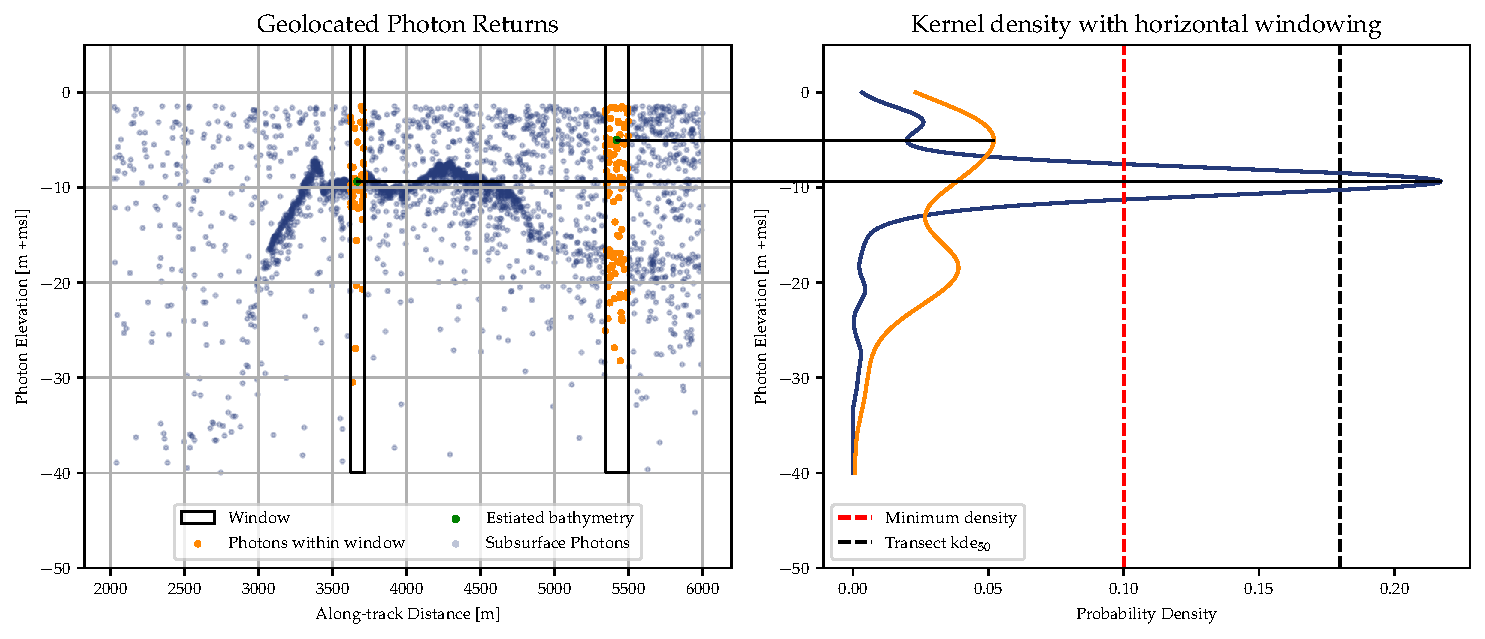
\includegraphics[width=\textwidth]{figures/2d_kde_plot.png}
    \caption{KDE function as applied to 2 different windows}
    \label{fig:kdefunc}
\end{figure}

The input parameters to the signal finding function are:

\begin{enumerate}
    \item The size of the window in \emph{number of points}
    \item the cutoff value for the Kernel Density required for point to be considered signal
\end{enumerate}

\subsection{Interpolation to a 2D grid}
After the bathymetric signal points are identified per the method in \ref{}, the resulting bathymetry points are densely spaced along satellite tracklines, but are absent between them. To convert these densely-spaced vector point locations to a raster of elevation data, and a raster of uncertainty data, geostatistical measures are used.

\subsubsection{Subsampling of Bathymetric points using Poisson Disk Sampling} \label{subsec:poissonsubsampling}
The bathymetric points are extremely densely spaced, and kriging algorithms are computationally expensive. To reduce the number of points fed into the algorithm, a subsample of the points is taken using the poisson disk sampling technique. 

\subsubsection{Kriging interpolation}
Using the subsample of the points from the poisson disk sampling, they are converted to a bathymetry raster using Universal Kriging. This geostatistical technique results in both a raster of the estimated depth as well as the estimated uncertainty. 


\subsection{Bayesian Data Assimilation using Kalman Filtering}
The Kalman Filter is a mathematical technique to predict the state of systems based on uncertain measurements. It consist of a loop of two steps, an \emph{Time update} step which updates the position based on a measurement and a known measurement uncertainty, and a \emph{measurement update} step which predicts the state based on the dynamic equations of the system. The kalman filter equations, for a state $x_k$ and a vector of measurements of the state $z_k$:

Time Update:

\begin{equation}
    \hat{x}_{\bar{k}} = A\hat{x}_{k-1} + B\hat{u_{k-1}}
\end{equation}

\begin{equation}
    P_{\bar{k}} = A P_{k-1} A^T + Q
\end{equation}

Measurement Update:
\begin{equation}
    K = P_{\bar{k}} H^T(H P_{\bar{k}} H^T + R) ^{-1}
\end{equation}

\begin{equation}
    \hat{x}_k = \hat{x}_{\bar{k}} + K(\hat{z}_k - H \hat{x}_{\bar{k}})
\end{equation}

\begin{equation}
    P_k = (I - KH)P_{\bar{k}}
\end{equation}


The coastal zone is a highly dynamic system. However, for the purposes of this project is is assumed that the temporal variations over the time scale being studied are within the margin of error of the measurements, so the bathymetry of the nearshore zone is assumed to be a static system and the time update step can be ignored. It is also assumed all measurements are measurements of the same underlying physical depth, and that differences between measurements are due to normally distributed measurement error, with magnitude of the error varying depending on the method. To combine multiple measurements, the \emph{measurement update} step is applied recursively for each available measurement, producing a bayesian estimate of the bathymetry.  

\subsection{Error Evaluation}
\pdfcomment{add RMSE error derivation}
\subsection{Case Studies}
